\chapter{Black-Hole Entropy, Holography, and de Sitter Space}

\lectureoverview{We complete the correspondence argument begun in the previous lecture. A highly excited string has an entropy proportional to its mass, while a Schwarzschild black hole has an entropy proportional to its area. The two formulas are connected not by identifying a strongly gravitating black hole with a free string, but by varying the string coupling slowly until the two descriptions meet. The area law then leads naturally to the holographic principle, and the final part of the lecture introduces expanding space and the de Sitter geometry whose horizon will be studied next.}

\section{Returning to the Counting Problem}

There was one loose end in the long-string count. If a fixed total length is divided among several strings, identical strings of the same length are indistinguishable. Their locations in the box are nevertheless part of the state, and the box is chosen to have roughly the size occupied by the corresponding single long string.

\begin{classroomqa}
\audiencequestion{Are the short strings distinguished from one another, and do their positions count?\lecturetimestamp{00:00:37}}
\lecturerresponse{Strings with identical properties are indistinguishable, but their positions in the box are counted. The comparison is made at fixed volume, chosen to match the region occupied by the long string.}
\end{classroomqa}

With that settled, we can state the target. We shall assemble a short list of equations and use them to obtain the scaling of black-hole entropy. No integral or infinite sum is required. The difficulty is not algebraic; it lies in knowing which quantities may be compared and at what stage of the argument.

\section{Natural Units and the Planck Area}

Set
\begin{equation}
c=\hbar=1,
\label{eq:l07-natural-units}
\end{equation}
but keep Newton's constant explicit. The first consequence is that time and length have the same units. The photon relation
\begin{equation}
E=\frac{\hbar c}{\lambda}
\end{equation}
and the mass-energy relation \(E=mc^2\) then imply
\begin{equation}
[M]=L^{-1}.
\label{eq:l07-mass-dimension}
\end{equation}
Mass can therefore be quoted as an inverse length.

\begin{figure}[htbp]
\centering

\includegraphics[width=0.62\textwidth]{lecture_07_figure_02.png}
\caption{The natural-units convention at the start of the dimensional argument. The energy formula is completed in the equations above.}
\lectureframe{00:03:27.900}
\end{figure}

To determine the units of \(G_N\), use Newtonian acceleration only as dimensional bookkeeping:
\begin{equation}
a\sim\frac{G_NM}{R^2}.
\end{equation}
Because \(T\) and \(L\) have the same units, \([a]=L/T^2=L^{-1}\). Together with Equation~\eqref{eq:l07-mass-dimension}, this gives
\begin{equation}
[G_N]=L^2.
\end{equation}
Newton's constant is an area in these units. Defining the Planck length by
\begin{equation}
G_N=\ell_p^2,
\label{eq:l07-planck-area}
\end{equation}
we immediately understand why \(A/G_N=A/\ell_p^2\) is dimensionless: it measures an area in Planck areas.

\section{The String Coupling and the Strength of Gravity}

Gravity must now be translated into string language. The useful picture is an exchange process. When a string crosses itself, it may split and rejoin. A small closed-string loop can be emitted by one object and absorbed by another; when that excitation is a graviton, the process mediates gravity. One interaction factor appears at emission and another at absorption, so the exchange strength contains \(g_s^2\).

The coupling \(g_s\) is dimensionless. More precisely, it is an amplitude-level coupling, while a probability or rate begins at order \(g_s^2\).\editorialnote{The lecture sometimes calls \(g_s\) a probability and then corrects this to the square root of a probability. The perturbative coupling belongs at amplitude level.} Since \(G_N\) has dimensions of area, a length scale is still missing. The fundamental string length \(\ell_s\), the scale of one elementary string wiggle, supplies it:
\begin{equation}
G_N\sim g_s^2\ell_s^2,
\qquad
\ell_p\sim g_s\ell_s.
\label{eq:l07-planck-string}
\end{equation}

\begin{figure}[htbp]
\centering

\includegraphics[width=0.72\textwidth]{lecture_07_figure_05.png}
\caption{The coupling relation on the board: \(G_N=\ell_p^2\) and \(g_s^2\ell_s^2\sim\ell_p^2\).}
\lectureframe{00:12:15.000}
\end{figure}

At weak coupling, \(g_s\ll1\), the Planck length is much smaller than the string length. Turning \(g_s\) down weakens gravity while leaving the elementary string scale fixed.\editorialnote{For an effective four-dimensional theory, compactification data and numerical conventions also enter \(G_N\). They are held fixed and suppressed in this scaling argument.}

\section{Counting a Long String}

Entropy counts the elementary decisions required to specify a state. Replace a highly excited string by a walk on a square lattice. At each vertex the next link may point in one of four directions. Whether the elementary choice is described as one four-way decision or two binary decisions changes only an order-one constant. What matters is the number of steps.

If \(L\) is the contour length of the string and each step has length \(\ell_s\), then
\begin{equation}
N=\frac{L}{\ell_s}
\end{equation}
steps are required. The number of walks grows exponentially, schematically \(\Omega_N\sim q^N\) with \(q\) of order unity, and hence
\begin{equation}
S_{\mathrm{str}}=\log\Omega_N\sim N\sim\frac{L}{\ell_s}.
\label{eq:l07-string-entropy-length}
\end{equation}

\begin{figure}[htbp]
\centering

\includegraphics[width=0.68\textwidth]{lecture_07_figure_03.png}

\vspace{0.7em}
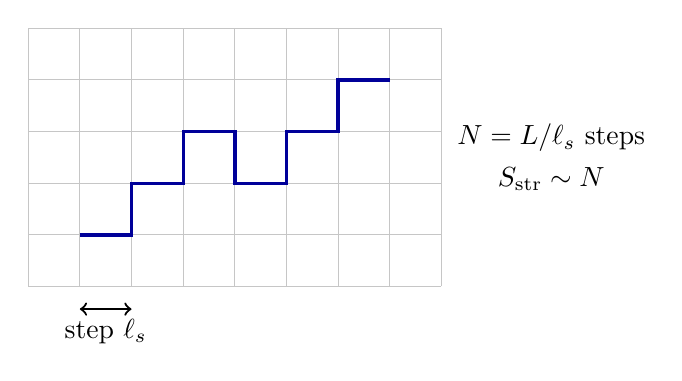
\begin{tikzpicture}[scale=0.82]
  \draw[step=0.8cm,gray!45,thin] (0,0) grid (6.4,4.0);
  \draw[very thick,blue!60!black]
    (0.8,0.8)--(1.6,0.8)--(1.6,1.6)--(2.4,1.6)--(2.4,2.4)--
    (3.2,2.4)--(3.2,1.6)--(4.0,1.6)--(4.0,2.4)--(4.8,2.4)--
    (4.8,3.2)--(5.6,3.2);
  \draw[<->,thick] (0.8,-0.35)--(1.6,-0.35);
  \node[below] at (1.2,-0.35) {step \(\ell_s\)};
  \node[align=center] at (8.1,2.0) {\(N=L/\ell_s\) steps\\[0.3em]\(S_{\mathrm{str}}\sim N\)};
\end{tikzpicture}
\caption{The lattice model on the board and its cleaned random-walk interpretation. The contour length, not the diameter of the tangled ball, determines the number of choices.}
\lectureframe{00:17:20.000}
\end{figure}

The mass is counted from the same elementary segments. A segment of length \(\ell_s\) has mass scale
\begin{equation}
m_{\mathrm{seg}}\sim\frac{1}{\ell_s}.
\end{equation}

\begin{classroomqa}
\audiencequestion{Is the elementary segment being assigned the length \(\ell_s\)?\lecturetimestamp{00:18:56}}
\lecturerresponse{Yes. Its characteristic length is \(\ell_s\), so in natural units its characteristic mass is \(1/\ell_s\).}
\end{classroomqa}

Adding the \(L/\ell_s\) segment masses gives
\begin{equation}
M\sim\frac{L}{\ell_s}\frac{1}{\ell_s}
=\frac{L}{\ell_s^2},
\qquad
L\sim M\ell_s^2.
\label{eq:l07-string-mass}
\end{equation}
The kinetic and potential energies of the oscillating string have been compressed into this scaling relation; a detailed statistical-mechanical treatment gives the same dependence. Substitution into Equation~\eqref{eq:l07-string-entropy-length} yields the string formula we shall need:
\begin{equation}
S_{\mathrm{str}}\sim M\ell_s.
\label{eq:l07-string-entropy-mass}
\end{equation}

\begin{figure}[htbp]
\centering

\includegraphics[width=0.66\textwidth]{lecture_07_figure_04.png}
\caption{The string-side column assembled before the comparison: \(\ell_p\sim g_s\ell_s\), \(S_{\mathrm{str}}\sim L/\ell_s\sim M\ell_s\), and \(M\sim L/\ell_s^2\).}
\lectureframe{00:21:57.800}
\end{figure}

\section{Why a Free String Is Not Yet a Black Hole}

On the gravitational side the exact semiclassical formula is
\begin{equation}
S_{\mathrm{BH}}=\frac{A}{4G_N}.
\label{eq:l07-bh-exact}
\end{equation}

\begin{classroomqa}
\audiencequestion{What numerical coefficient belongs in the denominator?\lecturetimestamp{00:23:28}}
\lecturerresponse{Four. The correspondence argument will recover the scaling but is too crude to determine that exact factor.}
\end{classroomqa}

For a four-dimensional Schwarzschild black hole,
\begin{equation}
R_s=2G_NM,
\qquad
A=4\pi R_s^2.
\end{equation}
Dropping numerical constants as the lecture does,
\begin{align}
S_{\mathrm{BH}}
&\sim\frac{A}{G_N}
\sim\frac{(G_NM)^2}{G_N} \\
&\sim M^2G_N
\sim M^2\ell_p^2.
\label{eq:l07-bh-scaling}
\end{align}

\begin{figure}[htbp]
\centering

\includegraphics[width=0.72\textwidth]{lecture_07_figure_06.png}
\caption{The completed comparison on the board: string entropy is a length in string units, whereas black-hole entropy is an area in Planck units.}
\lectureframe{00:25:35.000}
\end{figure}

The resemblance between Equations~\eqref{eq:l07-string-entropy-mass} and \eqref{eq:l07-bh-scaling} is suggestive, but they are not the same formula. It would be wrong simply to call the original black hole a free string and substitute. The free-string count omits the attractive interaction among the string's parts, precisely the interaction that compacts the string into a black hole and lowers its total energy through negative binding energy.

A star makes the error familiar. A hot gas of stellar mass placed in an oversized box is not a model of a star, even at the same temperature. Self-gravity changes the equilibrium size and the relation between energy and entropy. Following every self-interaction of a long string would be difficult, so we shall avoid doing so.

\begin{classroomqa}
\audiencequestion{If a small loop leaves a long string, its entropy decreases. Does graviton exchange therefore lower the entropy of the gravitating system?\lecturetimestamp{00:28:48}}
\lecturerresponse{Not in the equilibrium exchange process being used here. Virtual excitations are emitted and absorbed in both directions; the cartoon is not a literal loss of a permanent string fragment. Its only present purpose is to establish the two coupling factors and hence the \(g_s^2\) dependence.}
\end{classroomqa}

\section{The Adiabatic Correspondence Game}

Begin instead where gravity is negligible. At \(g_s\to0\), strings cross without splitting or joining and the self-gravitational attraction disappears. Increase \(g_s\) while holding \(\ell_s\) fixed: gravity strengthens, a highly excited string contracts, and eventually it becomes a black hole. Reverse the dial slowly and the black hole must return to a string state. It may become a small number of long strings, but the high-energy counting from the previous lecture says that the dominant sector contains one long string rather than an enormous gas of short ones.

\begin{classroomqa}
\audiencequestion{What is held fixed while the coupling is changed?\lecturetimestamp{00:32:19}}
\lecturerresponse{The string length \(\ell_s\), and therefore the elementary string mass scale \(1/\ell_s\), is held fixed. The dial changes \(g_s\) and hence \(G_N\sim g_s^2\ell_s^2\).}
\end{classroomqa}

The change must be slow, isolated, and reversible. Under those conditions entropy is an adiabatic invariant:
\begin{equation}
\Delta S=0.
\label{eq:l07-adiabatic}
\end{equation}
Slowness alone is not enough if dissipative or uncontrolled transitions occur. Here ``adiabatic'' means that the same family of states can be followed continuously.\editorialnote{This is the reversible thermodynamic sense of adiabatic. An irreversible process can be adiabatic in the no-heat-flow sense and still produce entropy.}

Let the target black hole have mass \(M_0\) and coupling \(g_{s,0}\). Before using the area formula we are trying to explain, dimensional analysis says only that the entropy of a neutral, nonrotating black hole is some function of the dimensionless combination
\begin{equation}
S_{\mathrm{BH}}=f(M\ell_p)
=f(Mg_s\ell_s).
\label{eq:l07-entropy-function}
\end{equation}
At fixed \(\ell_s\), an isentropic path therefore keeps
\begin{equation}
Mg_s=M_0g_{s,0}
\label{eq:l07-adiabat}
\end{equation}
constant, provided the same branch of states is followed.

As \(g_s\) decreases, negative binding energy is removed, so the mass \(M\) rises along this path. The underlying string configuration also becomes less tightly bound and spreads. The formal Schwarzschild radius, however, behaves as \(R_s\sim Mg_s^2\ell_s^2\sim g_s\ell_s\) on the adiabat and therefore decreases.\editorialnote{The spoken discussion uses ``grows'' for the object released from gravitational binding. It should not be read as saying that the Schwarzschild radius grows along the derived adiabat.}

\begin{classroomqa}
\audiencequestion{Does the object grow or shrink as gravity is weakened?\lecturetimestamp{00:36:28}}
\lecturerresponse{Its string structure is released and expands, while its mass increases because negative binding energy is removed. The radius assigned by the black-hole formula decreases until it reaches the string scale, where that black-hole description ceases to be useful.}
\end{classroomqa}

\section{Two Curves and Their Intersection}

Plot mass vertically and string coupling horizontally. Equation~\eqref{eq:l07-adiabat} is a hyperbola, \(M\propto g_s^{-1}\).

\begin{classroomqa}
\audiencequestion{What kind of curve has constant product \(Mg_s\)?\lecturetimestamp{00:44:08}}
\lecturerresponse{A hyperbola. It is the adiabat through the target point \((g_{s,0},M_0)\).}
\end{classroomqa}

The second curve marks the crossover between descriptions. A black hole cannot be resolved as a conventional Schwarzschild geometry once its radius is smaller than an elementary string wiggle. We therefore estimate the correspondence point by
\begin{equation}
R_s\sim\ell_s.
\label{eq:l07-correspondence-radius}
\end{equation}
Using \(R_s\sim MG_N\) and Equation~\eqref{eq:l07-planck-string}, this becomes
\begin{equation}
Mg_s^2\ell_s^2\sim\ell_s,
\qquad
Mg_s^2\sim\frac{1}{\ell_s}.
\label{eq:l07-transition-curve}
\end{equation}
Thus the transition curve falls as \(M\propto g_s^{-2}\), more steeply than the adiabat.

\begin{figure}[htbp]
\centering

\includegraphics[width=0.70\textwidth]{lecture_07_figure_07.png}

\vspace{0.6em}
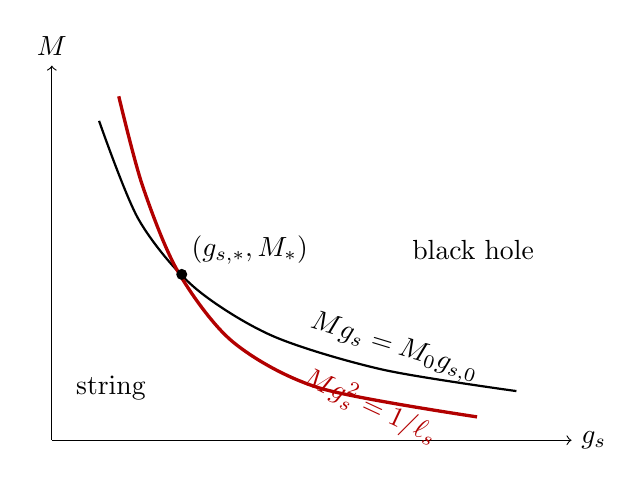
\begin{tikzpicture}[x=1cm,y=0.78cm]
  \draw[->] (0.4,0.4)--(7.0,0.4) node[right] {\(g_s\)};
  \draw[->] (0.4,0.4)--(0.4,6.5) node[above] {\(M\)};
  \draw[thick,black] plot[smooth] coordinates {(1.0,5.6) (1.5,4.0) (2.2,2.9) (3.2,2.1) (4.6,1.55) (6.3,1.2)};
  \draw[very thick,red!70!black] plot[smooth] coordinates {(1.25,6.0) (1.55,4.55) (2.0,3.15) (2.7,2.0) (3.8,1.25) (5.8,0.78)};
  \fill (2.05,3.1) circle (2pt) node[above right] {\((g_{s,*},M_*)\)};
  \node[black,rotate=-17] at (4.75,1.9) {\(Mg_s=M_0g_{s,0}\)};
  \node[red!70!black,rotate=-25] at (4.45,0.95) {\(Mg_s^2=1/\ell_s\)};
  \node at (5.75,3.5) {black hole};
  \node at (1.15,1.25) {string};
\end{tikzpicture}
\caption{The board graph and its cleaned interpretation. The black adiabat intersects the steeper red correspondence curve at the point where the object becomes string-like.}
\lectureframe{00:49:35.000}
\end{figure}

At the intersection \((M_*,g_{s,*})\), the two equations are
\begin{align}
M_*g_{s,*} &= M_0g_{s,0}, \\
M_*g_{s,*}^2 &\sim \frac{1}{\ell_s}.
\end{align}
Square the first equation and divide by the second:
\begin{equation}
M_*
\sim M_0^2g_{s,0}^2\ell_s.
\end{equation}
Multiplying by \(\ell_s\),
\begin{equation}
M_*\ell_s
\sim M_0^2g_{s,0}^2\ell_s^2
\sim M_0^2G_{N,0}.
\label{eq:l07-crossover-result}
\end{equation}

\begin{figure}[htbp]
\centering

\includegraphics[width=0.68\textwidth]{lecture_07_figure_08.png}
\caption{The completed crossover algebra, including \(M_*\ell_s=M_0^2g_{s,0}^2\ell_s^2=M_0^2G_{N,0}\).}
\lectureframe{00:54:40.000}
\end{figure}

\begin{classroomqa}
\audiencequestion{When the two curve equations are divided, should \(\ell_s\) end up upstairs or downstairs?\lecturetimestamp{00:52:41}}
\lecturerresponse{Upstairs. Dividing by \(1/\ell_s\) multiplies by \(\ell_s\), which is why \(M_*\sim M_0^2g_{s,0}^2\ell_s\).}
\end{classroomqa}

At the crossover the string formula is valid, so
\begin{equation}
S_*\sim M_*\ell_s.
\end{equation}
Entropy was unchanged along the path. Combining this statement with Equation~\eqref{eq:l07-crossover-result} gives the entropy of the original target black hole:
\begin{equation}
S_{\mathrm{BH}}(M_0)
\sim M_0^2G_{N,0}
\sim M_0^2\ell_{p,0}^2.
\label{eq:l07-final-correspondence}
\end{equation}
This is the desired area-law scaling.

\section{What the Correspondence Does and Does Not Prove}

The construction does not say that the original, strongly gravitating black hole is a free string. It moves the object to a regime where the string count is trustworthy, reads the entropy there, and carries that entropy back along a reversible path. The transition is a crossover rather than a sharply located phase boundary, so this estimate cannot determine the coefficient \(1/4\) in Equation~\eqref{eq:l07-bh-exact}.

The same logic nevertheless works parametrically for charged black holes, black objects in other dimensions, and extended black branes. More symmetric and supersymmetric examples permit protected state counts that retain exact information as the coupling changes; those methods recover numerical coefficients but add mathematical machinery not needed for the present conceptual argument.

Most importantly, the calculation supplies a microscopic interpretation. Entropy is evidence of hidden structure. Fluid mechanics describes density, pressure, and flow while omitting molecules; the fluid's entropy reveals that such microscopic degrees of freedom exist. General relativity similarly describes a horizon without displaying its microstates. The string count shows that a consistent quantum theory of gravity can contain enough states to account for the black-hole entropy.

\begin{classroomqa}
\audiencequestion{What would \(S\sim M^3\ell_p^3\) have meant instead of the quadratic result?\lecturetimestamp{00:59:41}}
\lecturerresponse{It would have looked like a volume law. Ordinary matter in a room or a cup of coffee has entropy proportional to volume; the quadratic answer is special because, through \(R_s\sim M\ell_p^2\), it is proportional to horizon area.}
\end{classroomqa}

The result is evidence that the Bekenstein--Hawking entropy is not merely a formal thermodynamic analogy. It points to microscopic gravitational degrees of freedom, even though the elementary derivation does not make those degrees of freedom visible one by one.

\section{From Maximum Entropy to Holography}

We now change the question. Instead of asking for the entropy of a specified state, ask for the greatest entropy compatible with a region.

Start with an ordinary lattice model of a room. Divide the volume into cells of size \(V_{\mathrm{cell}}\), and let each cell carry one yes-no question: occupied or empty. Susskind gives the imaginary atom the deliberately absurd name ``meatonium'' so that no realistic atomic details distract from the count. If
\begin{equation}
N=\frac{V}{V_{\mathrm{cell}}},
\end{equation}
then the number of configurations and the maximum entropy are
\begin{equation}
\Omega=2^N,
\qquad
S_{\max}=\log\Omega=N\log2
\sim\frac{V}{V_{\mathrm{cell}}}.
\label{eq:l07-volume-count}
\end{equation}

\begin{figure}[htbp]
\centering

\includegraphics[width=0.68\textwidth]{lecture_07_figure_09.png}
\caption{The room divided into cells, with two states per cell. This counts a maximum entropy, not the entropy of the orderly room occupied by the class.}
\lectureframe{01:05:20.000}
\end{figure}

The actual room is far below this maximum. A state that explored all those cell choices chaotically would be extremely hot. What survives from the toy model is the ordinary expectation that the number of independent degrees of freedom, and hence maximum entropy, scales with volume.

Gravity overturns that expectation. Consider a spherical region with boundary area \(A\), initial entropy \(S_{\mathrm{i}}\), and mass \(M\) below the mass \(M_{\mathrm{BH}}\) of a black hole that would just fill the sphere. If \(M\) were larger, its horizon would already extend beyond the chosen boundary.

Now send in a shell with mass \(M_{\mathrm{BH}}-M\). Its composition is irrelevant; the lecture allows light, ordinary matter, or even Swiss cheese. Arrange for it to collapse. The final state is a black hole whose horizon just fills the region, with entropy
\begin{equation}
S_{\mathrm{f}}=\frac{A}{4G_N}.
\end{equation}
The second law requires
\begin{equation}
S_{\mathrm{i}}\le S_{\mathrm{f}}
=\frac{A}{4G_N}.
\label{eq:l07-holographic-bound}
\end{equation}

\begin{figure}[htbp]
\centering

\includegraphics[width=0.70\textwidth]{lecture_07_figure_10.png}

\vspace{0.5em}
\begin{tikzpicture}[scale=0.88]
  \draw[thick] (0,0) circle (1.35);
  \draw[very thick,red!70!black] (0,0) circle (2.05);
  \fill[gray!25] (0,0) circle (1.32);
  \node at (0,0) {\(M,S_{\mathrm{i}}\)};
  \draw[-{Latex[length=3mm]},thick,red!70!black] (3.5,0)--(2.15,0);
  \node[align=center,right] at (3.5,0) {incoming shell\\\(M_{\mathrm{BH}}-M\)};
  \node[below] at (0,-2.2) {final horizon area \(A\)};
\end{tikzpicture}
\caption{The shell construction. Enough additional mass is sent inward to form a black hole whose horizon just fills the selected region.}
\lectureframe{01:13:30.000}
\end{figure}

Because a black hole of that size is an allowed state and saturates the inequality, the maximal entropy is
\begin{equation}
S_{\max}=\frac{A}{4G_N}.
\label{eq:l07-holographic-maximum}
\end{equation}
This is the holographic principle in its counting form: the maximum number of independent degrees of freedom in a gravitating region scales with the area of its boundary, approximately one order-unity degree of freedom per Planck area, rather than with the number of Planck volumes inside.\editorialnote{The shell argument assumes the region can be enclosed and collapsed in the stated way. More general spacetimes require covariant entropy bounds, but the spherical argument captures the principle used in the lecture.}

The disparity is enormous. Local field-theory intuition suggests that choices made at different interior points should combine independently, producing a volume law. Gravity says that sufficiently many such choices would themselves collapse, and the black hole supplies the larger admissible entropy. The boundary count is therefore not a small correction to the volume count; it is a different organization of the Hilbert space.

\begin{classroomqa}
\audiencequestion{What happens for a very large universe with roughly uniform density?\lecturetimestamp{01:15:48}}
\lecturerresponse{That question requires cosmology rather than the static spherical construction. It motivates the immediate turn to expanding solutions of Einstein's equations.}
\end{classroomqa}

\begin{classroomqa}
\audiencequestion{Is the area bound connected with the uncertainty principle?\lecturetimestamp{01:16:03}}
\lecturerresponse{The lecture leaves this question open and moves next to cosmology.}
\end{classroomqa}

\section{Expanding Space}

We shall not derive the cosmological solutions from Einstein's equations here; we shall write the solutions and learn how to read them. Spatial slices can be positively curved and closed, negatively curved and hyperbolic, or flat. For the present discussion take spatially flat Euclidean slices in a time-dependent spacetime.

\begin{classroomqa}
\audiencequestion{What is the spacetime analogue of ordinary Euclidean space?\lecturetimestamp{01:19:37}}
\lecturerresponse{Minkowski space. The cosmology considered here has flat spatial slices but is not Minkowski spacetime, because its spatial metric changes with time.}
\end{classroomqa}

The familiar balloon picture describes a closed expanding surface one dimension lower. Susskind recalls trying the demonstration with a large marked balloon; the marker weakened the rubber and produced a literal bang. The mishap also exposes a conceptual defect in the analogy. As an ordinary balloon expands, its rubber molecules separate and the material thins until it breaks. Cosmological space does not acquire diluted local laws. To preserve the analogy one must imagine continually inserting new rubber molecules so that every small patch retains the same local properties. In a flat model, replace the balloon by a large sheet pulled uniformly outward and similarly replenished.

Mathematically, the expansion belongs in the metric:
\begin{equation}
\begin{aligned}
ds^2&=-dt^2+a(t)^2d\mathbf{x}^2,\\
d\mathbf{x}^2&=\delta_{ij}\,dx^i dx^j
=dx^2+dy^2+dz^2.
\end{aligned}
\label{eq:l07-frw-metric}
\end{equation}

\begin{figure}[htbp]
\centering

\includegraphics[width=0.72\textwidth]{lecture_07_figure_11.png}
\caption{The spatially flat expanding metric as written on the board.}
\lectureframe{01:25:10.000}
\end{figure}

Points that keep fixed spatial coordinates are called comoving. If two such points have coordinate separation \(\Delta x\), their proper distance at time \(t\) is
\begin{equation}
D(t)=a(t)\Delta x.
\label{eq:l07-proper-distance}
\end{equation}
Their coordinates do not move, but the metric distance between them changes. Differentiating at fixed \(\Delta x\),
\begin{equation}
V=\dot D=\dot a\,\Delta x
=\frac{\dot a}{a}D.
\end{equation}
Define the Hubble parameter
\begin{equation}
H(t)=\frac{\dot a(t)}{a(t)}.
\label{eq:l07-hubble-parameter}
\end{equation}
Then
\begin{equation}
V=H(t)D,
\label{eq:l07-hubble-law}
\end{equation}
which is Hubble's law at a fixed cosmic time.

\begin{figure}[htbp]
\centering

\includegraphics[width=0.68\textwidth]{lecture_07_figure_12.png}
\caption{The equal-time recession law on the board: \(V=D\,\dot a/a\).}
\lectureframe{01:29:10.000}
\end{figure}

The name ``Hubble constant'' can mislead. In general \(H(t)\) changes with time. What is spatially constant is the ratio \(V/D\) for every pair of comoving points on the same time slice.

\begin{classroomqa}
\audiencequestion{For distant galaxies, whose time appears in this relation? We observe them at an earlier epoch.\lecturetimestamp{01:31:10}}
\lecturerresponse{Equation~\eqref{eq:l07-hubble-law} is an equal-time statement. An observation follows a past-directed light ray and samples the distant galaxy at an earlier time, so the relation between measured redshift and distance requires the full light-cone history rather than one instantaneous value of \(H\).}
\end{classroomqa}

\begin{figure}[htbp]
\centering

\includegraphics[width=0.66\textwidth]{lecture_07_figure_13.png}
\caption{The spacetime sketch used to distinguish an equal-time separation from what an observer sees along a past light ray.}
\lectureframe{01:33:20.000}
\end{figure}

\section{The Hubble Scale and de Sitter Expansion}

In units \(c=1\), Equation~\eqref{eq:l07-hubble-law} assigns recession speed one at the distance
\begin{equation}
D_H=\frac{1}{H}.
\label{eq:l07-hubble-radius}
\end{equation}
More distant comoving points can have \(V>1\), or even \(V\gg1\), without violating special relativity. They do not pass a local observer faster than light; their proper separation grows because the intervening geometry expands.\editorialnote{For a general time-dependent cosmology, \(1/H\) is the Hubble radius, not automatically an event horizon. It becomes the constant horizon scale in the de Sitter case discussed next.}

In many older decelerating cosmological models, \(H(t)\) decreases and \(1/H(t)\) grows, so regions once receding superluminally can later enter causal contact. The late-time picture discussed in the lecture instead approaches a positive constant \(H\). Then \(1/H\) remains fixed, and the expansion equation becomes
\begin{equation}
\frac{\dot a}{a}=H,
\qquad
\dot a=Ha.
\label{eq:l07-constant-h}
\end{equation}

\begin{classroomqa}
\audiencequestion{What are the units of a constant Hubble parameter?\lecturetimestamp{01:38:24}}
\lecturerresponse{Inverse time. Equivalently, with \(c=1\), it is inverse length. The quantity \(H^{-1}\) supplies both an expansion time and a distance scale; the lecture uses an order-of-magnitude example of about fifteen billion years.}
\end{classroomqa}

The solution of Equation~\eqref{eq:l07-constant-h} is
\begin{equation}
a(t)=a_0e^{Ht}.
\label{eq:l07-desitter-scale-factor}
\end{equation}

\begin{classroomqa}
\audiencequestion{What function has a rate of change proportional to itself?\lecturetimestamp{01:39:04}}
\lecturerresponse{An exponential. Thus the scale factor is \(a_0e^{Ht}\), while the spatial coefficient \(a(t)^2\) in the metric grows as \(e^{2Ht}\).}
\end{classroomqa}

\begin{figure}[htbp]
\centering

\includegraphics[width=0.70\textwidth]{lecture_07_figure_14.png}
\caption{The constant-\(H\) equations and their exponential solution on the board.}
\lectureframe{01:39:30.000}
\end{figure}

A spacetime with this exponential expansion is de Sitter space. Its constant Hubble scale produces an event horizon at finite proper distance. The geometry is in a sense the complement of the black-hole picture: an observer remains inside a cosmological horizon while sufficiently distant objects recede and can never send signals that catch the observer. A black-hole horizon hides an interior from an exterior observer; a de Sitter horizon hides the exterior of the observer's accessible patch. Unlike an ordinary evaporating black hole, the ideal de Sitter geometry is treated here as persisting. The comparison is only beginning here. The next lecture develops the horizon, its thermodynamics, and the puzzles it creates for cosmology.
